\chapter{Наблюдатель полного порядка}
\label{ch:chap2}
\section{Условие задачи}

Рассматреть систему:
$$
  \begin{cases}
    \dot{x} = Ax \\
    y = Cx
  \end{cases}
$$ и выполнить следующие шаги:

\begin{itemize}
    \item  Найти собственные числа матрицы $A$ и определить наблюдаемость каждого из них. 
    Сделать вывод об наблюдаемости и обнаруживаемости системы.
    \item  Построить схему моделирования системы с наблюдателем состояния $\dot{\hat{x}} = A\hat{x} + L(C\hat{x}-y  )$
    \item Для каждого из спектров:
    \begin{itemize}
        \item  Найти соответствующую матрицу коррекции наблюдателя $L$, обеспечивающую желаемый спектр.
        \item Определить собственные числа матрицы наблюдателя $(A+LC)$ и сравнить
        с желаемым спектром в подтверждение корректности синтеза наблюдателя.
        \item Выполнить компьютерное моделирование с начальными условиями системы 
        $x(0) = \begin{bmatrix} 1&1&1&1 \end{bmatrix}^T$ и наблюдателя $\hat{x}(0)=\begin{bmatrix}2 & 0& 0 &-1\end{bmatrix}^T $.
        Построить  сравнительные графики $x(t)$ и $\hat{x}(t)$, а также график ошибки наблюдателя
         $e(t) = x(t) - \hat{x}(t)$
    \end{itemize}
    \item Сопоставить полученные результаты компьютерного моделирования для рассмотренных спектров, 
    оценить возможные сравнительные преимущества и недостатки каждого из них.
\end{itemize}
    

\section{Решение задачи}

Параметры для объекта:
$$
  A = \begin{bmatrix}
    -40 & 16 & 9 & -7 \\
    -64 & 25 & 14 & -12 \\
    -26 & 11 & 7 & -3 \\
    48 & -18 & -14 & 8
  \end{bmatrix} \tab
  C = \begin{bmatrix}
    -7&-2&5&-3
  \end{bmatrix}
$$
И следующие спектры сходимости для синтеза наблюдателя:
$$
  \begin{aligned}
    \sigma_1 = \{-4,-4,-4,-4\} \\
    \sigma_2 = \{-4,-40,-400,-4000\} \\
    \sigma_3 = \{-4 \pm 5i, -4 \pm 6i\} 
  \end{aligned}
$$


\subsection{Исследование наблюдаемости системы}
Найдём собственные числа матрицы $A$:
$$
    \lambda_{1,2} = \pm 3i, \tab \lambda_{3,4} = \pm 2i,
$$
Можно заметить, что тут только комплексные моды, поэтому тип вектора состояния будет иметь колебательный характер.
Найдём матрицу наблюдаемости системы:
$$
V = \begin{bmatrix}
    C \\ CA \\ CA^2 \\ CA^3
\end{bmatrix} = \begin{bmatrix}
          -7     &     -2       &    5     &     -3 \\
        134      &   -53     &    -14       &   34 \\
          28    &     53   &     -110       &   12 \\
        -1076   &      347     &     56    &    -406

            \end{bmatrix}, \tab\rightarrow rank(V) = 4
$$

В таком случае по критерию Калмана - система полностью наблюдаема , а значит и все собственные числа наблюдаемы, и как следствие - система обнаруживаема.

Рассмотрим несколько вариантов синтеза наблюдателей, с разными спектрами:

\newpage
\begin{figure}[ht]
  \centering
  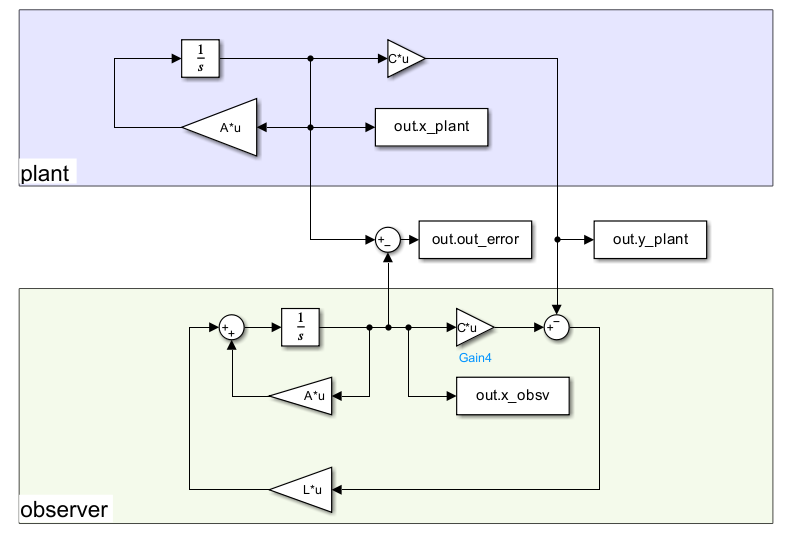
\includegraphics[width=0.8\textwidth]{model_observer.png}
  \caption{Модель с модальным наблюдателем}
\end{figure}

\subsection{Первый спектр}
$$
  \sigma_1 = \{-4,-4,-4,-4\}
$$
Система с наблюдателем полного порядка будет иметь следующие уравнения:
$$
\begin{cases}
  \dot{x} = Ax + Bu \\
  y = Cx 
\end{cases}, \tab 
\begin{cases}
  \dot{\hat{x}} = A\hat{x} + Bu +\mathbf{L}(\hat{y}-y)\\
  \hat{y} = C\hat{x} 
\end{cases}
$$

Для синтеза наблюдателя должны выполняться следующие условия:
$$
\begin{cases}
  \sigma(A)\cup\sigma(G)=\emptyset \\
  (G,Y) - \text{управляема, то всегда  существует } Q  \\
  (C,A) - \text{наблюдаема}
\end{cases}
$$
Тогда можно проследовать по алгоритму:
\begin{enumerate}
  \item Выбираем $G\in\mathbb{R}^{n\times n}$ с желаемым спектром $\sigma(G)$.
  \item Выбираем $Y\in\mathbb{R}^{n\times k}$ такую, чтобы пара $(G,Y)$ - была управляема.
  \item Найдем $Q\in\mathbb{R}^{n \times n}$ как решение уравнения Сильвестра $GQ - QA = YC$.
  \item Вычисляем матрицу коррекции наблюдателя: $L = Q^{-1}Y$
\end{enumerate}
Для получения $L$ возьмём следующую управляемую пару $G,Y$:
$$
G = \begin{bmatrix}
  -4  &   1  &   0  &   0 \\
  0  &  -4   &  1   &  0 \\
  0  &   0  &  -4  &   1 \\
  0   &  0   &  0  &  -4
\end{bmatrix}, \tab Y = \begin{bmatrix} 0\\1\\0\\1 \end{bmatrix},\tab \rightarrow \tab
L = \begin{bmatrix}
      11.08\\16.99\\9.74\\-15.62
    \end{bmatrix}
$$
Определим собственные числа матрицы наблюдателя $(A+LC)$:
$$
    \sigma_{obsv}=\{-4, -4, -4, -4 \}
$$
Однако я записал их в несколько округленном виде, поскольку мне не удалось подобрать удачный вектор $Y$, чтобы устранить такое отклонение:
$$
    \sigma_{true}=\{-4.0044, -4 + 0.0044i, -4 - 0.0044i, -3.9956 \}
$$
Но всё же погрежность здесь несколько незначительна, поэтому всё же сделаю вывод, что желаемые спектры совпали с спектром матрицы наблюдателя - синтез корректен.

Проведём моделирование, посмотрим на сравнительный график сходимости вектора состояния наблюдателя и системы, а также на их ошибку:
\newpage
\begin{figure}[ht]
  \centering
  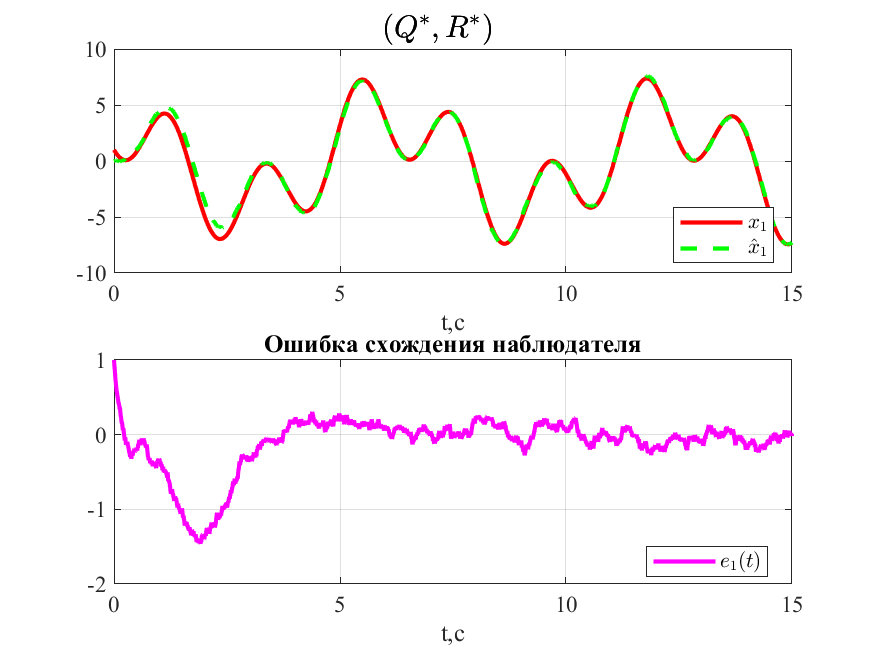
\includegraphics[width=0.8\textwidth]{obsv1.png}
  \caption{Состояние системы и ошибка сходимости}
\end{figure}
\begin{figure}[ht]
  \centering
  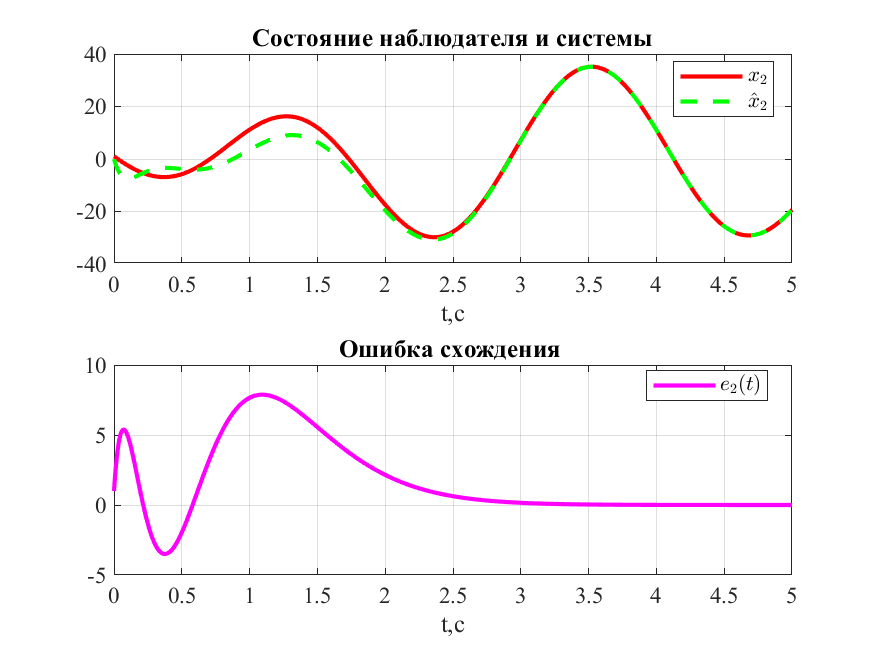
\includegraphics[width=0.8\textwidth]{obsv2.png}
  \caption{Состояние системы и ошибка сходимости}
\end{figure}
\newpage
\begin{figure}[ht]
  \centering
  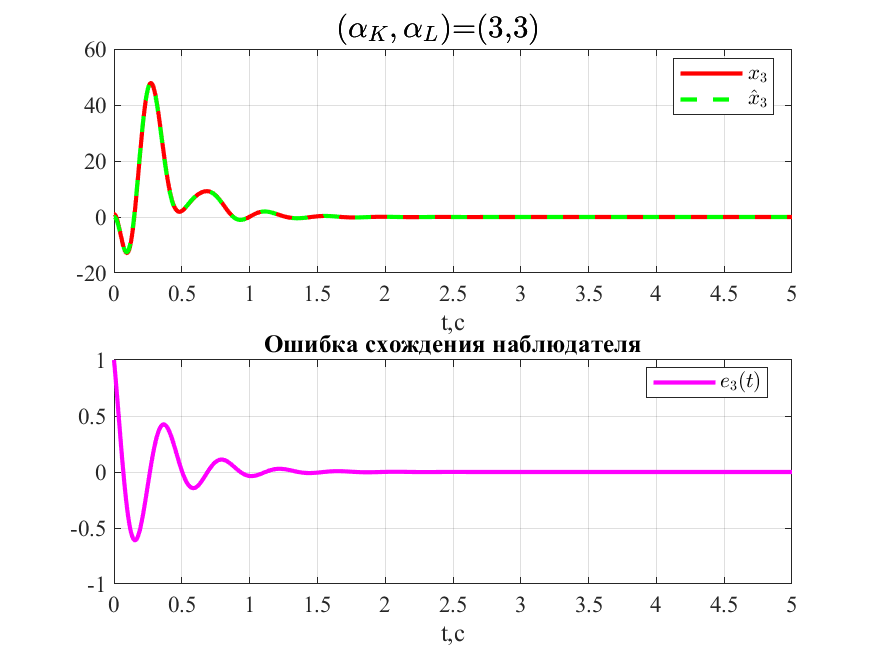
\includegraphics[width=0.8\textwidth]{obsv3.png}
  \caption{Состояние системы и ошибка сходимости}
\end{figure}
\begin{figure}[ht]
  \centering
  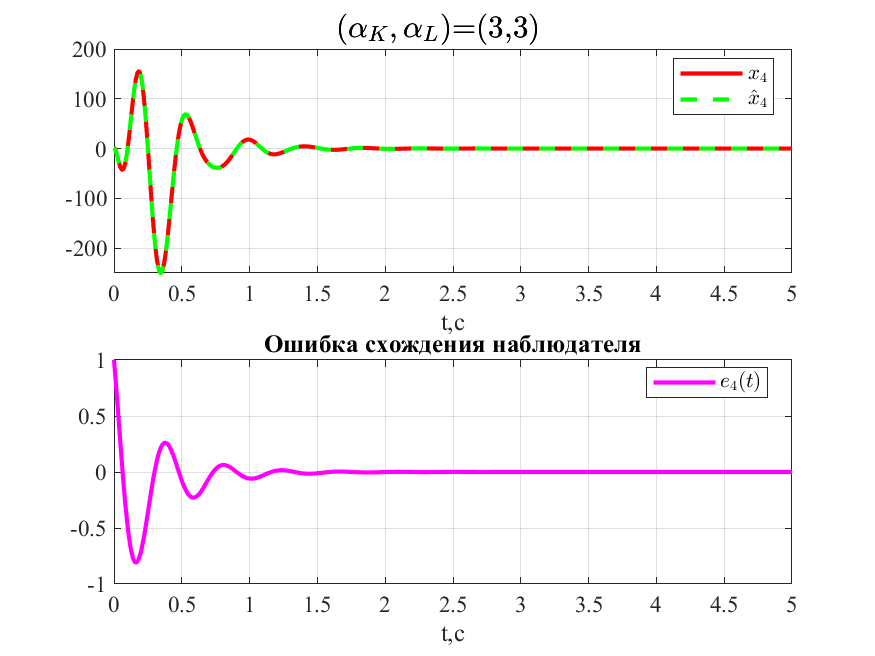
\includegraphics[width=0.8\textwidth]{obsv4.png}
  \caption{Состояние системы и ошибка сходимости}
\end{figure}


\newpage
\subsection{Второй спектр}
$$
  \sigma_2 = \{-4,-40,-400,-4000\}
$$

Для получения $L$ возьмём следующую управляемую пару $G,Y$:
$$
G = \begin{bmatrix}
  -4  &   0  &   0  &   0 \\
  0  &  -40   &  0   &  0 \\
  0  &   0  &  -400  &   0 \\
  0   &  0   &  0  &  -4000
\end{bmatrix}, \tab Y = \begin{bmatrix} 1\\1\\1\\1 \end{bmatrix},\tab \rightarrow \tab
L = 10^5\cdot\begin{bmatrix}
  3.157\\9.716\\12.754\\7.427
    \end{bmatrix}
$$
Определим собственные числа матрицы наблюдателя $(A+LC)$:
$$
    \sigma_{obsv}=\{-4, -40, -400, -4000 \}
$$
Можно сделать вывод, что желаемые спектры совпали с спектром матрицы наблюдателя - синтез корректен.
\begin{figure}[ht]
  \centering
  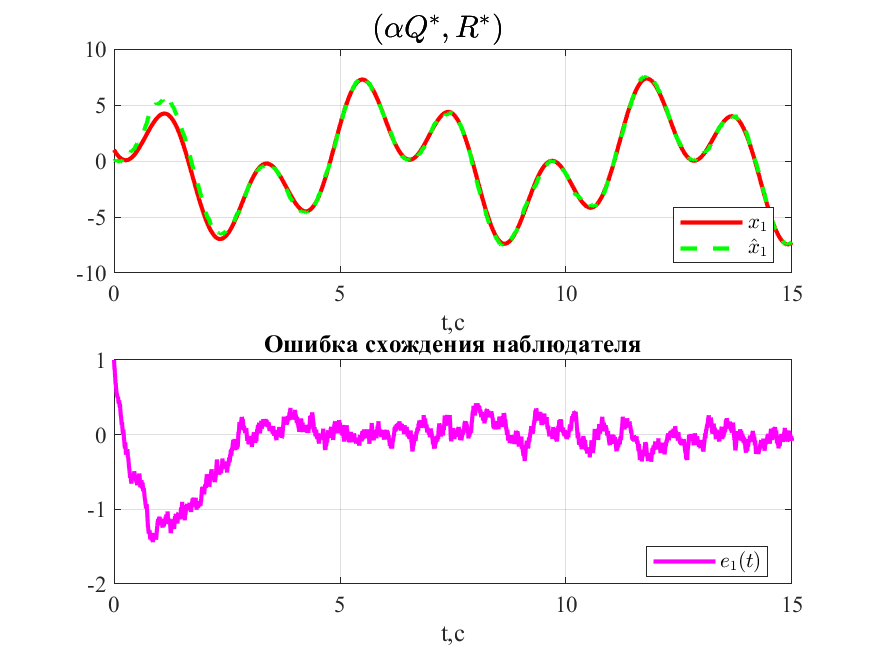
\includegraphics[width=0.8\textwidth]{obsv5.png}
  \caption{Состояние системы и ошибка сходимости}
\end{figure}
\newpage
\begin{figure}[ht]
  \centering
  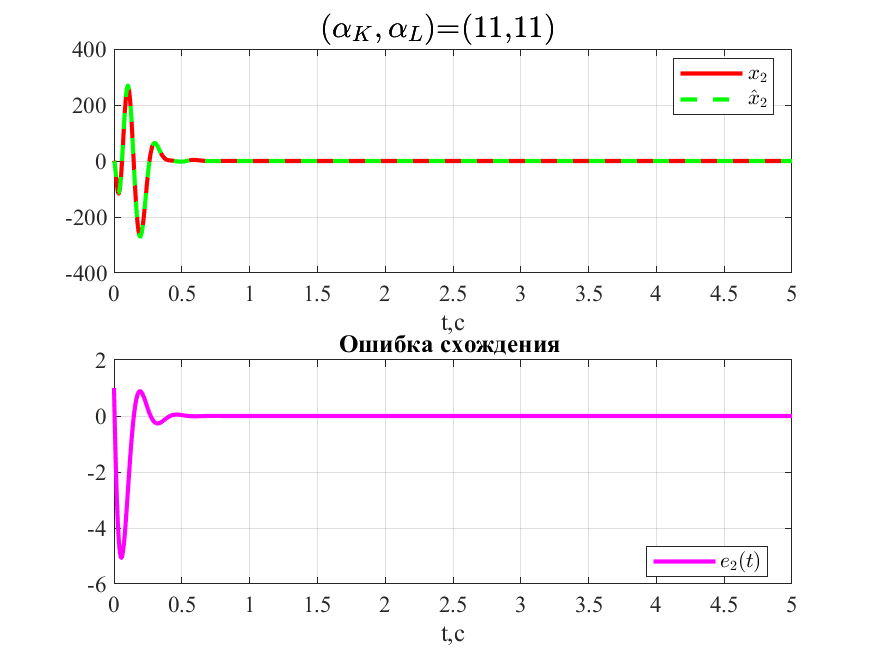
\includegraphics[width=0.8\textwidth]{obsv6.png}
  \caption{Состояние системы и ошибка сходимости}
\end{figure}
\begin{figure}[ht]
  \centering
  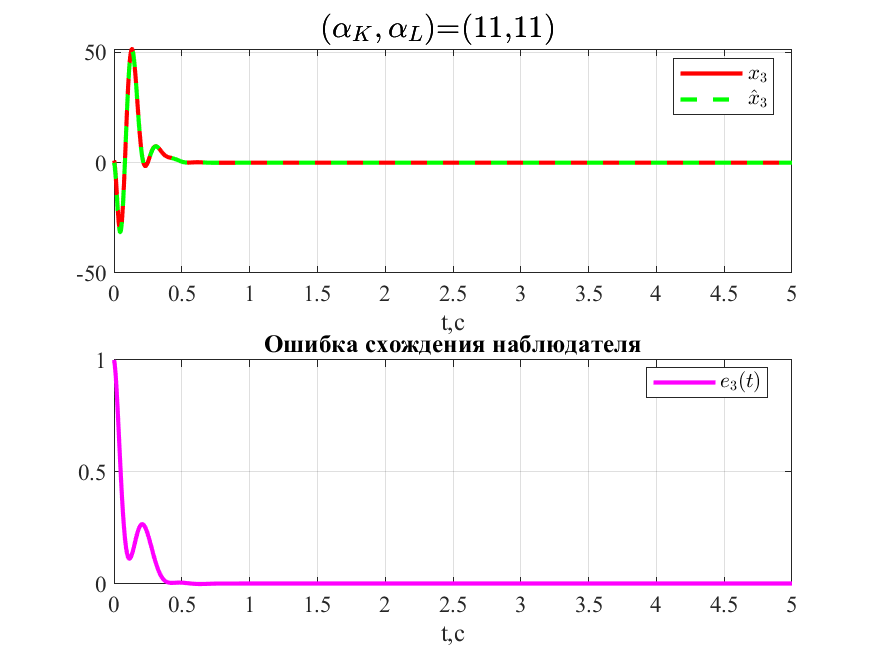
\includegraphics[width=0.8\textwidth]{obsv7.png}
  \caption{Состояние системы и ошибка сходимости}
\end{figure}
\newpage
\begin{figure}[ht]
  \centering
  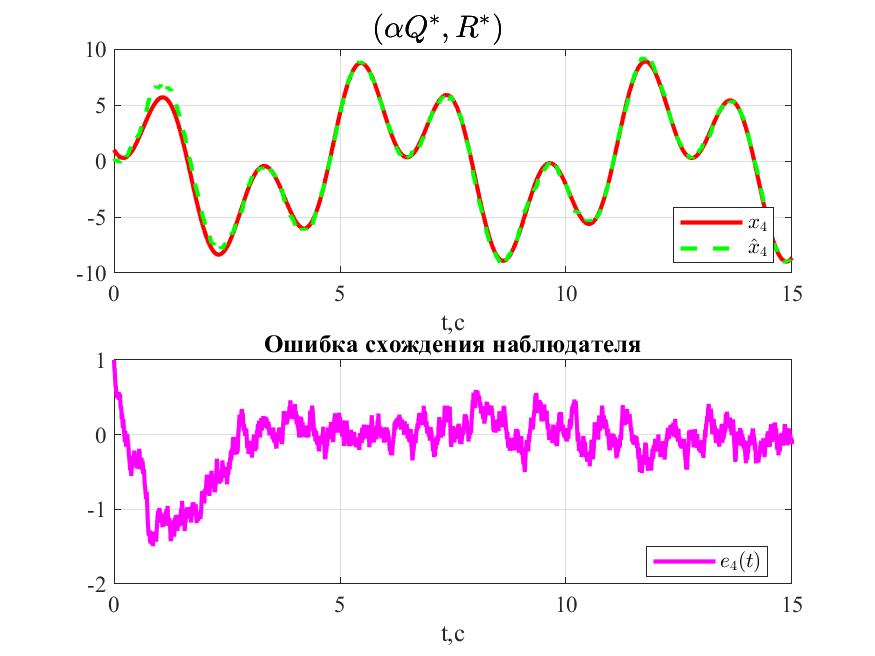
\includegraphics[width=0.8\textwidth]{obsv8.png}
  \caption{Состояние системы и ошибка сходимости}
\end{figure}


\newpage
\subsection{Третий спектр}
$$
  \sigma_3 = \{-4 \pm 5i, -4 \pm 6i\} 
$$

Для получения $L$ возьмём следующую управляемую пару $G,Y$:
$$
G = \begin{bmatrix}
  -4  &   5  &   0  &   0 \\
  -5  &  -4   &  0   &  0 \\
  0  &   0  &  -4  &   6 \\
  0   &  0   &  -6  &  -4
\end{bmatrix}, \tab Y = \begin{bmatrix} 0\\1\\0\\1 \end{bmatrix},\tab \rightarrow \tab
L = \begin{bmatrix}
  14.56\\25.87\\19.60\\-13.23
    \end{bmatrix}
$$
Определим собственные числа матрицы наблюдателя $(A+LC)$:
$$
    \sigma_{obsv}=\{-4 \pm 5i, -4 \pm 6i\}
$$
Можно сделать вывод, что желаемые спектры совпали с спектром матрицы наблюдателя - синтез корректен.
Проведём моделирование:
\begin{figure}[ht]
  \centering
  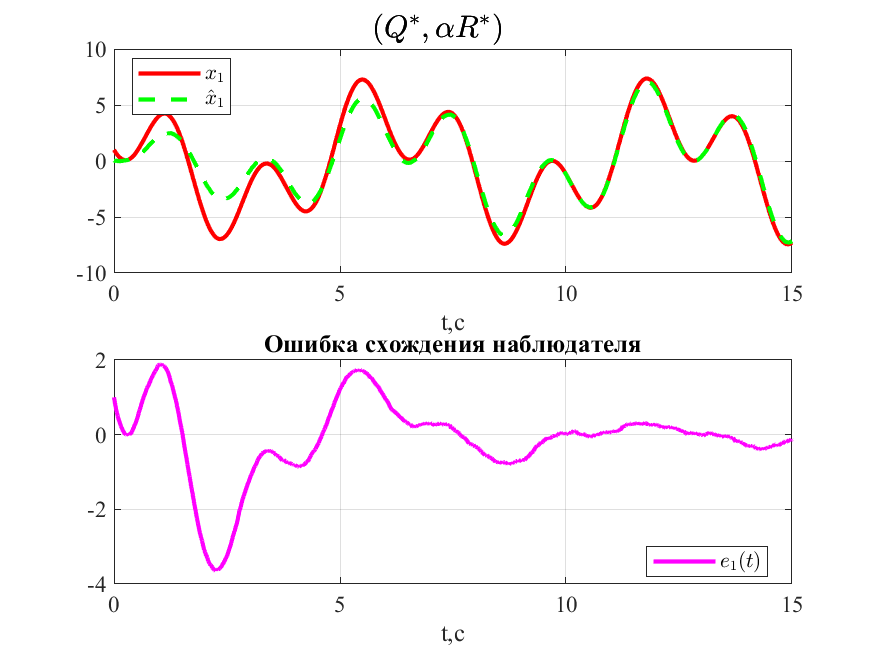
\includegraphics[width=0.8\textwidth]{obsv9.png}
  \caption{Состояние системы и ошибка сходимости}
\end{figure}
\newpage
\begin{figure}[ht]
  \centering
  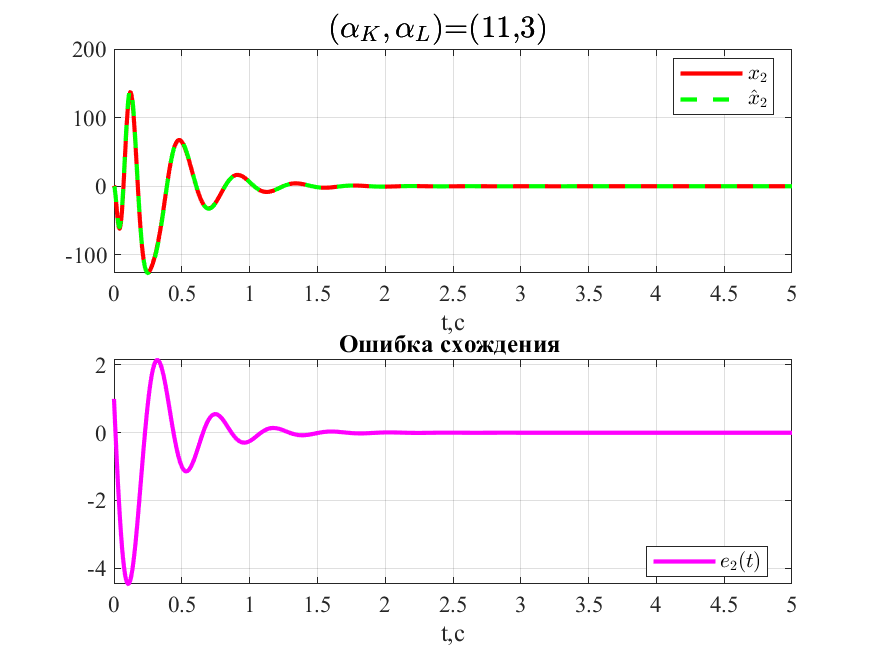
\includegraphics[width=0.8\textwidth]{obsv10.png}
  \caption{Состояние системы и ошибка сходимости}
\end{figure}
\begin{figure}[ht]
  \centering
  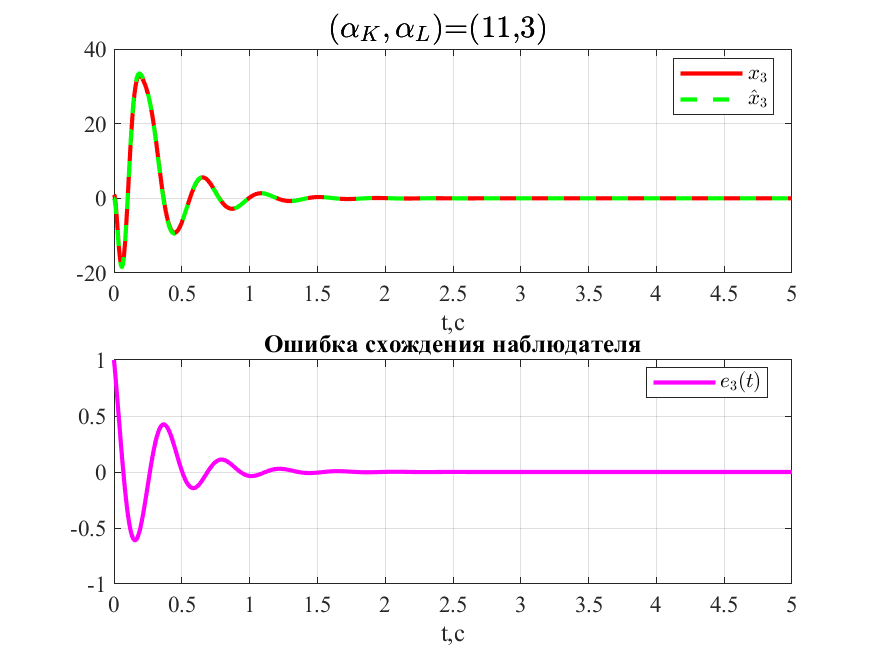
\includegraphics[width=0.8\textwidth]{obsv11.png}
  \caption{Состояние системы и ошибка сходимости}
\end{figure}
\newpage
\begin{figure}[ht]
  \centering
  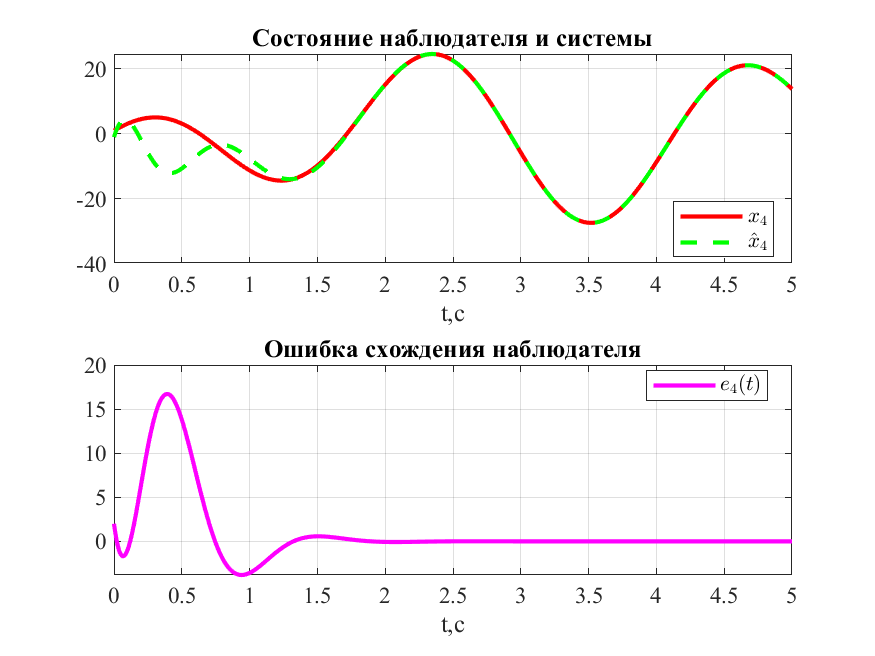
\includegraphics[width=0.8\textwidth]{obsv12.png}
  \caption{Состояние системы и ошибка сходимости}
\end{figure}


\newpage
\subsection{Сравнение выбора собственных чисел для синтеза наблюдателя}
Мы можем заметить, что происходят похожие процессы, как и при синтезе модального регулятора - выбор мод наблюдателя напрямую влияет на характер его схождения к истинной системе.
В первом случае спектр выбран не слишком большим, поэтому матрица коррекции не слишком велика, в итоге мы получили довольно большое перерегулирование (по графику ошибки) при небольшом времени переходного процесса.

Во втором случае мы получили довольно агрессивную сходимость(перерегулирования практически нет, время переходного процесса экстремально мало), но в реальных физических системах вряд ли
наша оценка может так быстро/резки сойтись к истинной безошибочно, 
потому что датчики шумные, и их фильтрация стоит какого-то времени на сбор достаточного количества данных, и последующуб обработку.

В третьем случае наш спектр состоял в том числе и из колебательных мод, поэтому переходный процесс был с перерегулированием куда больше, чем в первом случае, однако время этого процесса стало куда меньше.

\subsection{Вывод}
В этом задании мы работали с полностью наблюдаемой системой, это мы узнали через критерий Калмана.
Мы узнали, что синтезировать наблюдатели можно с разным "характером" сходимости. Для наблюдения мы 
синтезировали модального наблюдателя с помощью уравнения Сильвестра, а также провели серию моделирований с разными наблюдателями, все они показали то, 
что мы сходимся к оригинальной системе с разным качеством переходного процесса - его времени и перерегулирования.
\endinput 